\documentclass{standalone}
\usepackage{tikz}
\usetikzlibrary{patterns, positioning}

\begin{document}
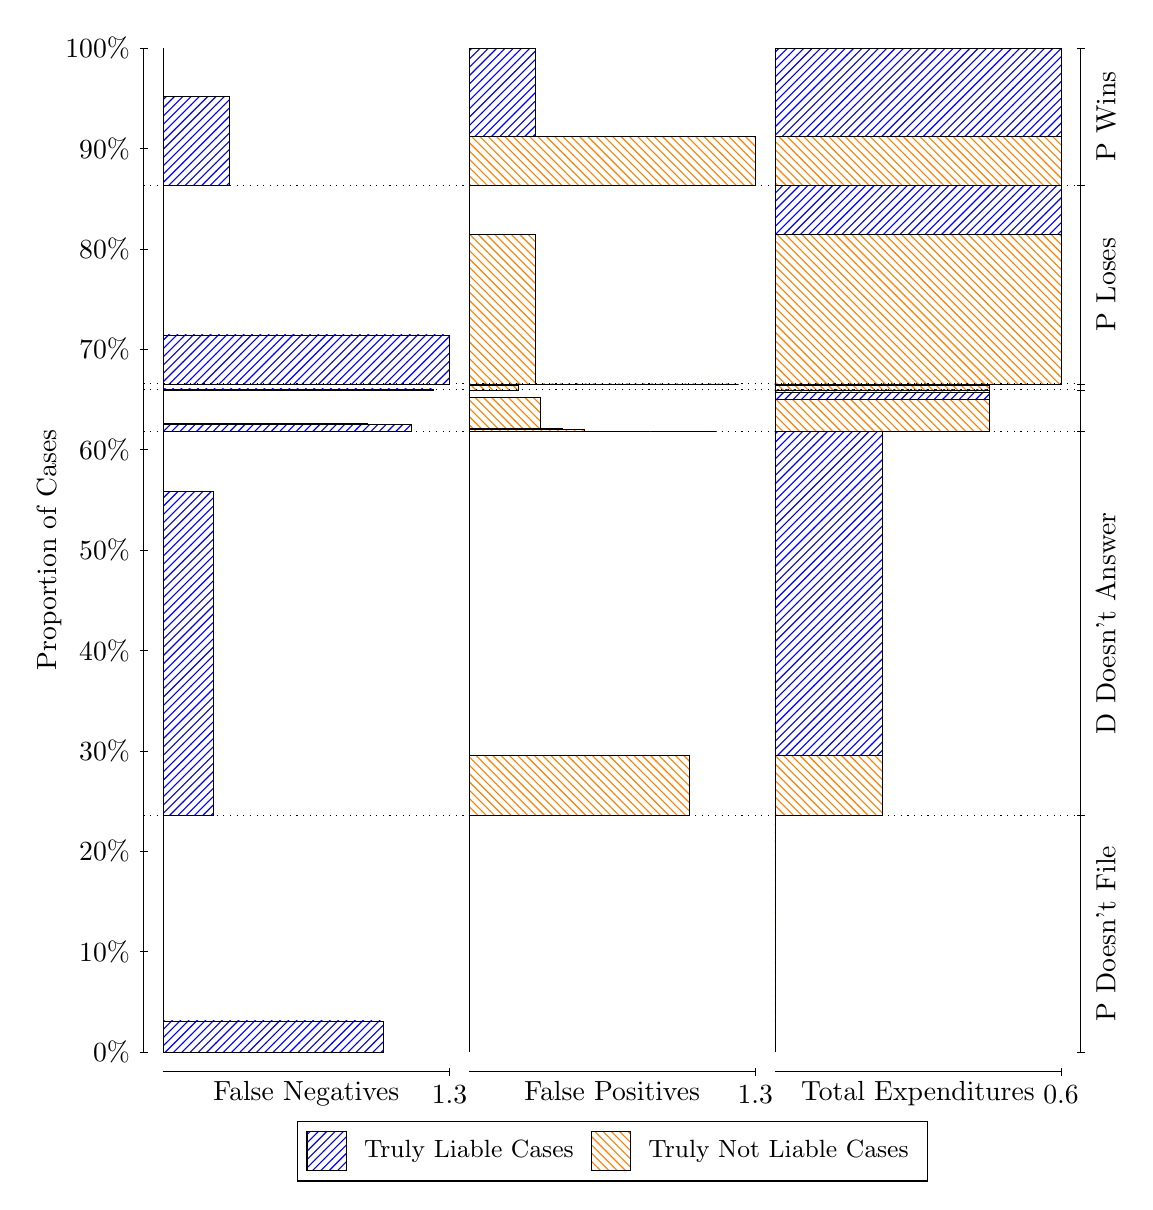
\begin{tikzpicture}
\draw[black, very thin] (1.5,1.75) -- (1.5,14.5);
\node[rotate=90, anchor=center] at (0.3, 8.125) {Proportion of Cases};
\draw[black, very thin] (1.45,1.75) -- (1.55,1.75);
\node[anchor=east] at (1.45, 1.75) {0\%};
\draw[black, very thin] (1.45,3.025) -- (1.55,3.025);
\node[anchor=east] at (1.45, 3.025) {10\%};
\draw[black, very thin] (1.45,4.3) -- (1.55,4.3);
\node[anchor=east] at (1.45, 4.3) {20\%};
\draw[black, very thin] (1.45,5.575) -- (1.55,5.575);
\node[anchor=east] at (1.45, 5.575) {30\%};
\draw[black, very thin] (1.45,6.85) -- (1.55,6.85);
\node[anchor=east] at (1.45, 6.85) {40\%};
\draw[black, very thin] (1.45,8.125) -- (1.55,8.125);
\node[anchor=east] at (1.45, 8.125) {50\%};
\draw[black, very thin] (1.45,9.4) -- (1.55,9.4);
\node[anchor=east] at (1.45, 9.4) {60\%};
\draw[black, very thin] (1.45,10.675) -- (1.55,10.675);
\node[anchor=east] at (1.45, 10.675) {70\%};
\draw[black, very thin] (1.45,11.95) -- (1.55,11.95);
\node[anchor=east] at (1.45, 11.95) {80\%};
\draw[black, very thin] (1.45,13.225) -- (1.55,13.225);
\node[anchor=east] at (1.45, 13.225) {90\%};
\draw[black, very thin] (1.45,14.5) -- (1.55,14.5);
\node[anchor=east] at (1.45, 14.5) {100\%};

\draw[black, very thin] (13.4,1.75) -- (13.4,14.5);
\draw[black, very thin] (13.35,1.75) -- (13.45,1.75);
\node[anchor=west] at (13.35, 1.75) {};
\draw[black, very thin] (13.35,4.7509) -- (13.45,4.7509);
\node[anchor=west] at (13.35, 4.7509) {};
\draw[black, very thin] (13.35,9.6352) -- (13.45,9.6352);
\node[anchor=west] at (13.35, 9.6352) {};
\draw[black, very thin] (13.35,10.158) -- (13.45,10.158);
\node[anchor=west] at (13.35, 10.158) {};
\draw[black, very thin] (13.35,10.236) -- (13.45,10.236);
\node[anchor=west] at (13.35, 10.236) {};
\draw[black, very thin] (13.35,10.236) -- (13.45,10.236);
\node[anchor=west] at (13.35, 10.236) {};
\draw[black, very thin] (13.35,12.757) -- (13.45,12.757);
\node[anchor=west] at (13.35, 12.757) {};
\draw[black, very thin] (13.35,14.5) -- (13.45,14.5);
\node[anchor=west] at (13.35, 14.5) {};

\draw[black, very thin, pattern color=blue, pattern=north east lines] (1.75,1.75) rectangle (4.5449,2.1446);
\draw[black, very thin, pattern color=orange, pattern=north west lines] (1.75,2.1446) rectangle (1.75,4.7509);
\draw[black, very thin, pattern color=blue, pattern=north east lines] (1.75,4.7509) rectangle (2.3788,8.8722);
\draw[black, very thin, pattern color=orange, pattern=north west lines] (1.75,8.8722) rectangle (1.75,9.6352);
\draw[black, very thin, pattern color=blue, pattern=north east lines] (1.75,9.6352) rectangle (4.8942,9.7172);
\draw[black, very thin, pattern color=blue, pattern=north east lines] (1.75,9.7172) rectangle (4.6147,9.7242);
\draw[black, very thin, pattern color=blue, pattern=north east lines] (1.75,9.7242) rectangle (4.3353,9.7337);
\draw[black, very thin, pattern color=blue, pattern=north east lines] (1.75,9.7337) rectangle (4.0558,9.7337);
\draw[black, very thin, pattern color=blue, pattern=north east lines] (1.75,9.7337) rectangle (3.7763,9.7338);
\draw[black, very thin, pattern color=blue, pattern=north east lines] (1.75,9.7338) rectangle (3.4968,9.7338);
\draw[black, very thin, pattern color=blue, pattern=north east lines] (1.75,9.7338) rectangle (3.2173,9.7338);
\draw[black, very thin, pattern color=blue, pattern=north east lines] (1.75,9.7338) rectangle (2.9378,9.7338);
\draw[black, very thin, pattern color=blue, pattern=north east lines] (1.75,9.7338) rectangle (2.6583,9.7338);
\draw[black, very thin, pattern color=orange, pattern=north west lines] (1.75,9.7338) rectangle (1.75,10.158);
\draw[black, very thin, pattern color=blue, pattern=north east lines] (1.75,10.158) rectangle (5.1737,10.172);
\draw[black, very thin, pattern color=orange, pattern=north west lines] (1.75,10.172) rectangle (1.75,10.236);
\draw[black, very thin, pattern color=blue, pattern=north east lines] (1.75,10.236) rectangle (2.3788,10.236);
\draw[black, very thin, pattern color=orange, pattern=north west lines] (1.75,10.236) rectangle (1.75,10.236);
\draw[black, very thin, pattern color=blue, pattern=north east lines] (1.75,10.236) rectangle (5.3833,10.857);
\draw[black, very thin, pattern color=orange, pattern=north west lines] (1.75,10.857) rectangle (1.75,12.757);
\draw[black, very thin, pattern color=blue, pattern=north east lines] (1.75,12.757) rectangle (2.5885,13.883);
\draw[black, very thin, pattern color=orange, pattern=north west lines] (1.75,13.883) rectangle (1.75,14.5);
\draw[black, very thin, pattern color=orange, pattern=north west lines] (5.6333,1.75) rectangle (5.6333,4.3563);
\draw[black, very thin, pattern color=blue, pattern=north east lines] (5.6333,4.3563) rectangle (5.6333,4.7509);
\draw[black, very thin, pattern color=orange, pattern=north west lines] (5.6333,4.7509) rectangle (8.4282,5.5139);
\draw[black, very thin, pattern color=blue, pattern=north east lines] (5.6333,5.5139) rectangle (5.6333,9.6352);
\draw[black, very thin, pattern color=orange, pattern=north west lines] (5.6333,9.6352) rectangle (8.7776,9.6352);
\draw[black, very thin, pattern color=orange, pattern=north west lines] (5.6333,9.6352) rectangle (8.4981,9.6352);
\draw[black, very thin, pattern color=orange, pattern=north west lines] (5.6333,9.6352) rectangle (8.2186,9.6352);
\draw[black, very thin, pattern color=orange, pattern=north west lines] (5.6333,9.6352) rectangle (7.9391,9.6352);
\draw[black, very thin, pattern color=orange, pattern=north west lines] (5.6333,9.6352) rectangle (7.6596,9.6354);
\draw[black, very thin, pattern color=orange, pattern=north west lines] (5.6333,9.6354) rectangle (7.3801,9.6354);
\draw[black, very thin, pattern color=orange, pattern=north west lines] (5.6333,9.6354) rectangle (7.1006,9.6564);
\draw[black, very thin, pattern color=orange, pattern=north west lines] (5.6333,9.6564) rectangle (6.8212,9.6718);
\draw[black, very thin, pattern color=orange, pattern=north west lines] (5.6333,9.6718) rectangle (6.5417,10.059);
\draw[black, very thin, pattern color=blue, pattern=north east lines] (5.6333,10.059) rectangle (5.9827,10.059);
\draw[black, very thin, pattern color=blue, pattern=north east lines] (5.6333,10.059) rectangle (5.7032,10.059);
\draw[black, very thin, pattern color=blue, pattern=north east lines] (5.6333,10.059) rectangle (5.6333,10.158);
\draw[black, very thin, pattern color=orange, pattern=north west lines] (5.6333,10.158) rectangle (6.2622,10.222);
\draw[black, very thin, pattern color=blue, pattern=north east lines] (5.6333,10.222) rectangle (5.6333,10.236);
\draw[black, very thin, pattern color=orange, pattern=north west lines] (5.6333,10.236) rectangle (9.0571,10.236);
\draw[black, very thin, pattern color=blue, pattern=north east lines] (5.6333,10.236) rectangle (6.2622,10.236);
\draw[black, very thin, pattern color=orange, pattern=north west lines] (5.6333,10.236) rectangle (6.4718,12.137);
\draw[black, very thin, pattern color=blue, pattern=north east lines] (5.6333,12.137) rectangle (5.6333,12.757);
\draw[black, very thin, pattern color=orange, pattern=north west lines] (5.6333,12.757) rectangle (9.2667,13.374);
\draw[black, very thin, pattern color=blue, pattern=north east lines] (5.6333,13.374) rectangle (6.4718,14.5);
\draw[black, very thin, pattern color=orange, pattern=north west lines] (9.5167,1.75) rectangle (9.5167,4.3563);
\draw[black, very thin, pattern color=blue, pattern=north east lines] (9.5167,4.3563) rectangle (9.5167,4.7509);
\draw[black, very thin, pattern color=orange, pattern=north west lines] (9.5167,4.7509) rectangle (10.879,5.5139);
\draw[black, very thin, pattern color=blue, pattern=north east lines] (9.5167,5.5139) rectangle (10.879,9.6352);
\draw[black, very thin, pattern color=orange, pattern=north west lines] (9.5167,9.6352) rectangle (12.242,9.6352);
\draw[black, very thin, pattern color=blue, pattern=north east lines] (9.5167,9.6352) rectangle (12.242,9.6352);
\draw[black, very thin, pattern color=orange, pattern=north west lines] (9.5167,9.6352) rectangle (12.242,10.038);
\draw[black, very thin, pattern color=blue, pattern=north east lines] (9.5167,10.038) rectangle (12.242,10.127);
\draw[black, very thin, pattern color=orange, pattern=north west lines] (9.5167,10.127) rectangle (12.242,10.148);
\draw[black, very thin, pattern color=blue, pattern=north east lines] (9.5167,10.148) rectangle (12.242,10.158);
\draw[black, very thin, pattern color=orange, pattern=north west lines] (9.5167,10.158) rectangle (12.242,10.158);
\draw[black, very thin, pattern color=blue, pattern=north east lines] (9.5167,10.158) rectangle (12.242,10.158);
\draw[black, very thin, pattern color=orange, pattern=north west lines] (9.5167,10.158) rectangle (12.242,10.222);
\draw[black, very thin, pattern color=blue, pattern=north east lines] (9.5167,10.222) rectangle (12.242,10.236);
\draw[black, very thin, pattern color=orange, pattern=north west lines] (9.5167,10.236) rectangle (12.242,10.236);
\draw[black, very thin, pattern color=blue, pattern=north east lines] (9.5167,10.236) rectangle (12.242,10.236);
\draw[black, very thin, pattern color=orange, pattern=north west lines] (9.5167,10.236) rectangle (13.15,12.137);
\draw[black, very thin, pattern color=blue, pattern=north east lines] (9.5167,12.137) rectangle (13.15,12.757);
\draw[black, very thin, pattern color=orange, pattern=north west lines] (9.5167,12.757) rectangle (13.15,13.374);
\draw[black, very thin, pattern color=blue, pattern=north east lines] (9.5167,13.374) rectangle (13.15,14.5);
\draw[black, dotted] (1.5,4.7509) -- (13.4,4.7509);
\draw[black, dotted] (1.5,9.6352) -- (13.4,9.6352);
\draw[black, dotted] (1.5,10.158) -- (13.4,10.158);
\draw[black, dotted] (1.5,10.236) -- (13.4,10.236);
\draw[black, dotted] (1.5,10.236) -- (13.4,10.236);
\draw[black, dotted] (1.5,12.757) -- (13.4,12.757);
\draw[black, very thin] (1.75,1.5) -- (5.3833,1.5);
\node[anchor=north] at (3.5667, 1.5) {False Negatives};
\draw[black, very thin] (5.3833,1.45) -- (5.3833,1.55);
\node[anchor=north] at (5.3833, 1.45) {1.3};

\draw[black, very thin] (5.6333,1.5) -- (9.2667,1.5);
\node[anchor=north] at (7.45, 1.5) {False Positives};
\draw[black, very thin] (9.2667,1.45) -- (9.2667,1.55);
\node[anchor=north] at (9.2667, 1.45) {1.3};

\draw[black, very thin] (9.5167,1.5) -- (13.15,1.5);
\node[anchor=north] at (11.333, 1.5) {Total Expenditures};
\draw[black, very thin] (13.15,1.45) -- (13.15,1.55);
\node[anchor=north] at (13.15, 1.45) {0.6};

\node[black, centered, rotate=90] at (13.72, 3.2505) {P Doesn't File};
\node[black, centered, rotate=90] at (13.72, 7.1931) {D Doesn't Answer};



\node[black, centered, rotate=90] at (13.72, 11.497) {P Loses};
\node[black, centered, rotate=90] at (13.72, 13.629) {P Wins};

\draw (7.449999999999999,1.5) node[draw=none] (baseCoordinate) {};
\begin{scope}[align=center]
        \matrix[scale=0.5, draw=black, below=0.5cm of baseCoordinate, nodes={draw}, column sep=0.1cm]{
            \node[rectangle, draw, minimum width=0.5cm, minimum height=0.5cm, pattern=north east lines, pattern color=blue] {}; &
            \node[draw=none, font=\small] (B) {Truly Liable Cases}; &
            \node[rectangle, draw, minimum width=0.5cm, minimum height=0.5cm, pattern=north west lines, pattern color=orange] {}; &
            \node[draw=none, font=\small] (B) {Truly Not Liable Cases}; \\
            };
\end{scope}

\end{tikzpicture}
\end{document}